\documentclass[11pt]{article}
\usepackage[margin=1in]{geometry}
\usepackage{graphicx}
\usepackage{booktabs}
\usepackage{float}
\usepackage{amsmath}

\title{2VG3 Homework 6 Written Answers}
\author{}
\date{}

\begin{document}
\maketitle

\section*{Exercise 1}
I completed the sequential impulse solver in \texttt{rigidbody2d\_seq.py}. The solver now:
\begin{itemize}
    \item stores the total normal impulse and total friction impulse per contact,
    \item iterates over all contacts many times each frame,
    \item clamps the total normal impulse so contacts only push apart,
    \item clamps friction to the static/kinetic friction cone, and
    \item applies a velocity bias term of the form
    \[
    v_{\text{bias}} = d_{\text{close}} \, \beta / \Delta t
    \]
    with the lecture default $\beta = 0.3$ still present in the code, while allowing smaller tuned values for the harder stack/bounce tests.
\end{itemize}

\section*{Exercise 2}
\subsection*{(a) Scenario 0: block on incline, gravity on, $e=0.05$, $\mu_s=\mu_k=0.5$}
With the sequential solver active, the block comes to rest on the incline instead of continuously creeping downhill. There is still a very small residual drift from the bias term and finite timestep, but it is tiny once enough iterations are used.

\subsection*{(b) Scenario 1: flat plane, gravity off, straight down velocity, $e=0$}
The block stops cleanly after impact once the sequential solver has enough iterations. This is a good sanity check because the final velocity should be zero, and there is no gravity to hide errors.

\subsection*{Iteration study}
For the simple two-body tests, I found that about 20 iterations was the minimum I would call ``good''. Below that, the second contact keeps undoing the first contact correction, so the block keeps some sideways drift and angular velocity.

\begin{table}[H]
\centering
\caption{Exercise 2 iteration sweep. To reproduce these rows in the terminal, run \texttt{\detokenize{python.exe rigidbody2d_seq.py --scenario 0 --exercise2-table}} and \texttt{\detokenize{python.exe rigidbody2d_seq.py --scenario 1 --exercise2-table}}.}
\begin{tabular}{@{}rll@{}}
\toprule
Iterations & Scenario 0 result & Scenario 1 result \\
\midrule
1   & speed $=0.0981$, obvious slide/spin & speed $=0.2161$, still bouncing/spinning \\
2   & speed $=0.0562$, still sliding & speed $=0.1970$, still not settled \\
5   & speed $=0.0123$, nearly stopped & speed $=0.0089$, nearly stopped \\
10  & speed $=0.0111$, small creep remains & speed $=4.6\times 10^{-4}$ \\
20  & speed $=0.0079$, acceptable & essentially zero velocity \\
50+ & visually same as 20 for these cases & essentially zero velocity \\
\bottomrule
\end{tabular}
\end{table}

What goes wrong for small iteration counts is exactly the multi-contact problem from the lecture: one contact correction creates a rotation that makes the other contact wrong again. In practice, the box slides, jitters, and spins instead of satisfying both contact constraints together.

\section*{Exercise 3}

To verify the results of this exercise in the terminal, run
\texttt{\detokenize{python.exe rigidbody2d_seq.py --headless --scenario 2 --frames 240 --report}}
and
\texttt{\detokenize{python.exe rigidbody2d_seq.py --headless --scenario 3 --frames 240 --report}}.
The program prints an \texttt{EX3\_METRIC} line that shows the incoming velocity, outgoing velocity, and the ideal reversed target velocity.

\subsection*{(a) Scenario 2: inclined plane bounce, gravity off, $e=1$}
This case bounced back essentially exactly along the incoming direction. After 240 frames the block velocity was approximately $(0.1, 0, 0.994987)$, which is the expected reversal of the initial $(-0.1, 0, -0.994987)$.

\subsection*{(b) Scenario 3: flat plane bounce, gravity off, $e=1$}
This case also behaved correctly: after impact, the velocity became approximately $(0,0,1)$, which is the exact reversal of the original straight-down velocity.

\subsection*{Energy check}
Using 120 iterations, both elastic bounce tests preserved total energy to the precision printed by the program:
\begin{itemize}
    \item Scenario 2: energy before collision $=0.500000$, after collision $=0.500000$.
    \item Scenario 3: energy before collision $=0.500000$, after collision $=0.500000$.
\end{itemize}
To verify this explicitly in the terminal, run
\texttt{\detokenize{python.exe rigidbody2d_seq.py --headless --scenario 2 --frames 240 --report}}
or
\texttt{\detokenize{python.exe rigidbody2d_seq.py --headless --scenario 3 --frames 240 --report}}.
The program prints an \texttt{EX3\_ENERGY} line with the energy before collision, energy after collision, the absolute change, the relative error, and a simple pass/fail value.
So, for these simple elastic tests, the sequential impulse implementation is doing the right thing.

\section*{Exercise 4}
\subsection*{Scenario 4: repeated bounce, gravity on, flat plane, $e=1$, no friction}
This case is the clearest demonstration of the velocity bias side effect. With a small tuned bias ($\beta = 0.005$, slope $=0.015$), the block keeps bouncing, but the total mechanical energy slowly rises:
\begin{itemize}
    \item initial total energy $=5.50$,
    \item final total energy after 900 frames $=6.77$.
\end{itemize}

So the qualitative behaviour is correct (it keeps bouncing), but the bias injects energy because every overlap correction adds a little extra outward speed. I also tried the lecture default $\beta = 0.3$ for this case; then the total energy exploded to about $195.6$ after 900 frames, so the energy growth is overwhelmingly caused by the bias term.

To print these values in the terminal, run \texttt{\detokenize{python.exe rigidbody2d_seq.py --headless --scenario 4 --frames 900 --report}}. To reproduce the lecture-default bias comparison, run \texttt{\detokenize{python.exe rigidbody2d_seq.py --headless --scenario 4 --frames 900 --report --bias-factor 0.3 --bias-slop 0.015}}.
The program prints an \texttt{EX4\_METRIC} line with the bias settings, initial total energy, final total energy, and total energy drift.

\section*{Exercise 5}
\subsection*{(a) Scenario 5: 5-box stack on inclined plane}
I used the lecture-style off-centre stack and tuned only solver parameters, not the physical setup. The best result I found was:
\begin{itemize}
    \item 400 iterations,
    \item bias factor $\beta = 0.05$,
    \item bias slop $=0.01$.
\end{itemize}

These values gave the cleanest stable stack I found: low jitter, no catastrophic squeezing, and no boxes shooting out of the pile. By the end of the run, all box speeds were only about $0.008$, so the stack had essentially settled.

For comparison:
\begin{itemize}
    \item 180 iterations with the stronger default bias were unstable and launched boxes out of the stack.
    \item 300 iterations with a smaller bias were already stable.
    \item 400 iterations gave the best overall result I found.
\end{itemize}

\begin{figure}[H]
\centering
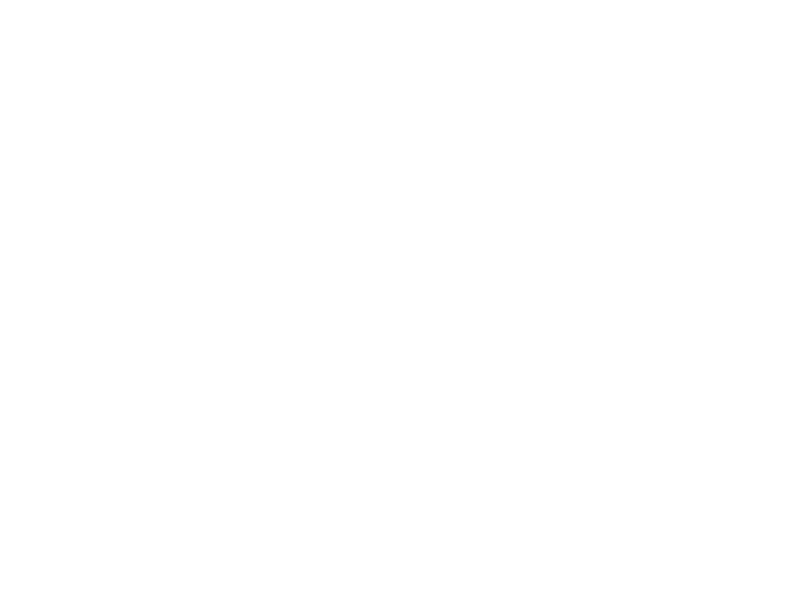
\includegraphics[width=0.68\linewidth]{hw6_scenario5.png}
\caption{Best stable stack found for scenario 5.}
\end{figure}

\subsection*{(b) Scenario 6: moving-frame stack}
Repeating the same setup with everything moving left at speed $-1$ produced essentially the same stack behaviour. The boxes stayed stacked while all of their $x$-velocities remained very close to $-1.0$ (roughly between $-0.9992$ and $-0.9975$ at the end of the run). That is a good Galilean invariance check: the simulation looks like scenario 5 plus a constant frame translation.

To print these values in the terminal, run
\texttt{\detokenize{python.exe rigidbody2d_seq.py --headless --scenario 5 --frames 1200 --report}} and \texttt{\detokenize{python.exe rigidbody2d_seq.py --headless --scenario 6 --frames 1200 --report}}. The program prints \texttt{EX5\_METRIC} and \texttt{EX6\_METRIC} lines with the iteration count, bias settings, final speed range, and final $x$-velocity range.

To inspect the scenario 5 comparison cases above, reuse the same command with \texttt{\detokenize{--niter 180 --bias-factor 0.3 --bias-slop 0.005}} for the unstable case or \texttt{\detokenize{--niter 300 --bias-factor 0.05 --bias-slop 0.01}} for the smaller-bias stable case.

\end{document}
